\section{Data collection from inertial sensors, magnetometer and GPS module}
\subsection{Collecting data from the accelerometer sensor}
\subsubsection{Accelerometer data rate}
The accelerometer data rate is $0.01$ seconds.
\subsubsection{Acceleration measurement mechanism in a MEMS accelerometer}
Microelectromechanical Systems (MEMS) accelerometers employ a capacitive sensing mechanism to measure acceleration. The basic working principle involves the movement of a proof mass in response to acceleration, leading to a change in capacitance. Here's a simplified explanation of the acceleration measurement mechanism in a MEMS accelerometer:

\begin{enumerate}
  \item \textbf{Proof Mass:} MEMS accelerometers have a small proof mass suspended within the device, anchored to the device structure by flexible springs.

  \item \textbf{Capacitor Structure:} The proof mass and the surrounding structure form a parallel plate capacitor. The capacitance between these plates changes as the distance between them changes due to the movement of the proof mass.

  \item \textbf{Acceleration Sensing:} When the accelerometer experiences acceleration, the proof mass moves in response to the force applied, changing the gap between the proof mass and the surrounding structure.

  \item \textbf{Capacitance Change:} The change in the gap results in a change in capacitance. As the proof mass moves, the capacitance between the proof mass and the surrounding structure varies.

  \item \textbf{Sensing Circuit:} The accelerometer is integrated with a sensing circuit that measures the capacitance changes, converting them into an electrical signal proportional to the applied acceleration.

  \item \textbf{Output Signal:} The electrical signal generated by the sensing circuit is processed and amplified to provide an output voltage or current representing the applied acceleration.

  \item \textbf{Interpretation:} The output signal is further processed and interpreted to determine the acceleration magnitude and direction. Calibration and compensation techniques may be employed to improve accuracy and reduce errors.

  \item \textbf{Types of MEMS Accelerometers:} Different types of MEMS accelerometers, including single-axis, dual-axis, and tri-axis devices, exist depending on the number of dimensions in which they can measure acceleration.
\end{enumerate}


\subsubsection{Specific Force}

Accelerometers measure specific forces denoted as \(f_{BI}\), representing forces experienced by the device in the Body frame (B) relative to the Inertial frame (I). Several fundamental reasons support the choice of measuring specific forces, rooted in physics principles and practical applications.

\begin{enumerate}
  \item \textbf{Reference Frame Independence:}
    By measuring specific forces, accelerometers provide a reference frame-independent measurement. This ensures that the accelerometer output reflects actual forces regardless of the device's orientation or motion.

  \item \textbf{Isolation of Gravitational Effects:}
    Measuring specific forces allows for the isolation of dynamic components from the static gravitational component. Accelerometers can distinguish between forces due to gravity and forces due to acceleration or motion.

  \item \textbf{Consistency Across Orientations:}
    Specific force measurements provide consistent results regardless of the accelerometer's orientation. This consistency is crucial for applications where the device may experience various orientations.

  \item \textbf{Inertial Navigation Systems (INS):}
    In applications like inertial navigation systems, accelerometers measure specific forces to determine changes in velocity and position accurately. This enables precise navigation calculations.

  \item \textbf{Simplicity in Calibration:}
    Calibrating accelerometers for specific forces simplifies the calibration process. Calibration parameters can be determined based on the device's response to known accelerations, remaining valid regardless of orientation.

  \item \textbf{Consistency with Newton's Laws:}
    Accelerometers measure forces based on Newton's second law (\(F = ma\)). Measuring specific forces directly captures the acceleration component, consistent with the fundamental principles of classical mechanics.
\end{enumerate}

\subsubsection{Accelerometer data}
The accelerometer data is shown in the figure \ref{fig:accelerometer_data}.
\begin{figure}[H]
  \centering
  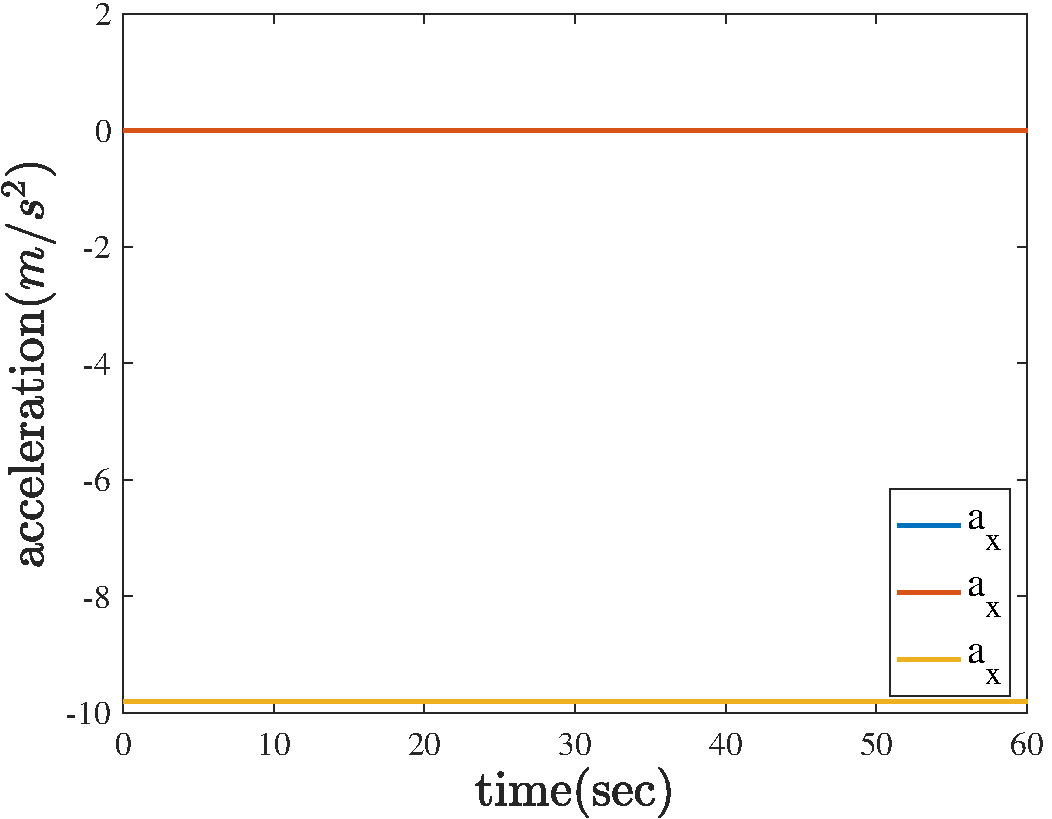
\includegraphics[width=0.8\textwidth]{../Figure/Q1/immovability}
  \caption{Accelerometer data}
  \label{fig:accelerometer_data}
\end{figure}
The direction of acceleration measured by an accelerometer when at rest is opposite to the Earth's gravitational field. This phenomenon is rooted in the fundamental principle of how accelerometers work and the conventions used in defining coordinate systems.

Accelerometers measure proper acceleration, including both the acceleration due to gravity and any additional accelerations. In the absence of external acceleration (e.g., when the device is stationary), the only acceleration detected is due to gravity.

The convention for defining the direction of gravitational acceleration typically involves assigning the positive direction opposite to the gravitational field. Consequently, when the gravitational field points downward, the accelerometer measures an upward acceleration, and vice versa. The numerical value is denoted as \(g\) (approximately 9.8 $m/s²$ on the Earth's surface).

Consider a scenario where the accelerometer is at rest and not experiencing any external acceleration. Since the only acceleration it detects is due to gravity, the measured acceleration is equal in magnitude to \(g\) but in the opposite direction. Mathematically, if the accelerometer measures acceleration as \(a\), it is expressed as \(-g\) in the opposite direction.

This sign convention is crucial for maintaining consistency in various applications, especially in inertial navigation and motion analysis, where understanding the direction of gravity is essential for accurate measurements and calculations.

\subsubsection{Roll and pitch angles}

  The roll and pitch angles are shown in the figure \ref{fig:roll_pitch_angles} and \ref{fig:roll_pitch_angles_2}
The roll and pitch angles are calculated using the following equations:
\begin{equation}
  \phi = \arctan{\frac{a_y}{a_z}}
\end{equation}
\begin{equation}
  \theta = \arctan{\frac{-a_x}{\sqrt{a_y^2 + a_z^2}}}
\end{equation}

\begin{figure}[H]
  \centering
  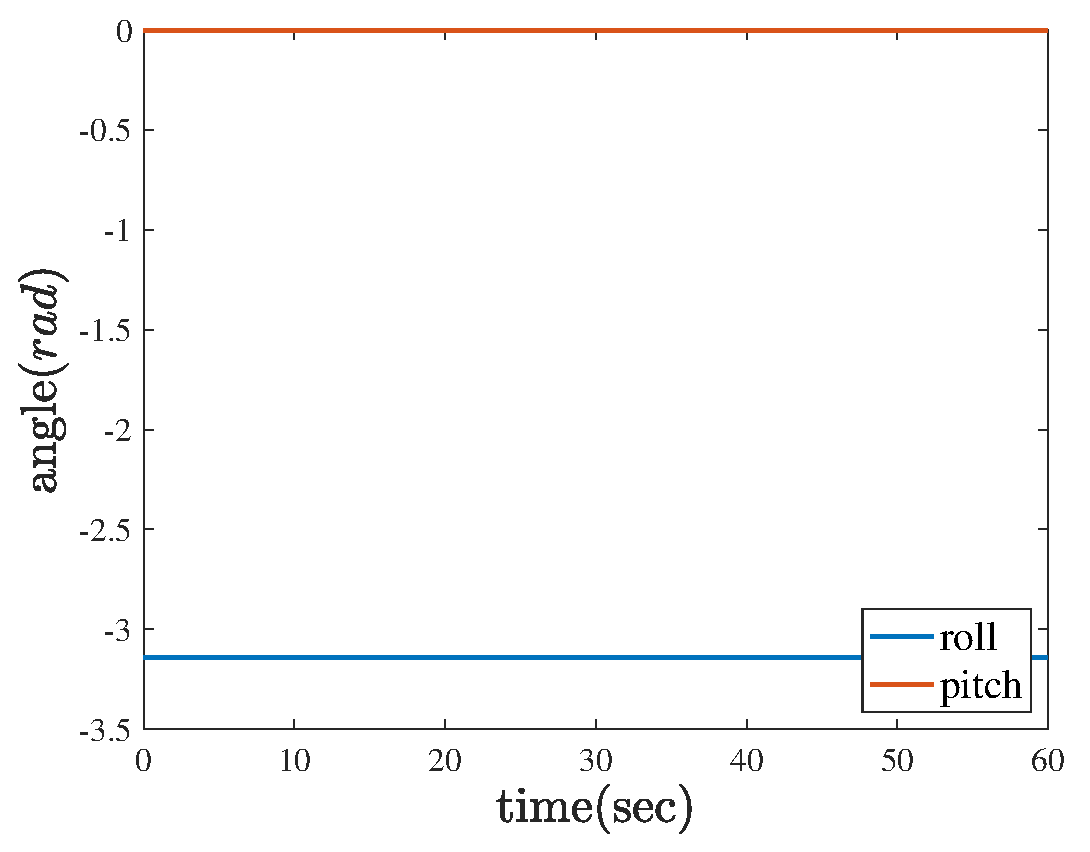
\includegraphics[width=0.8\textwidth]{../Figure/Q1/roll_pitch}
  \caption{Roll and pitch angles in scenario I}
  \label{fig:roll_pitch_angles}
\end{figure}

\begin{figure}[H]
  \centering
  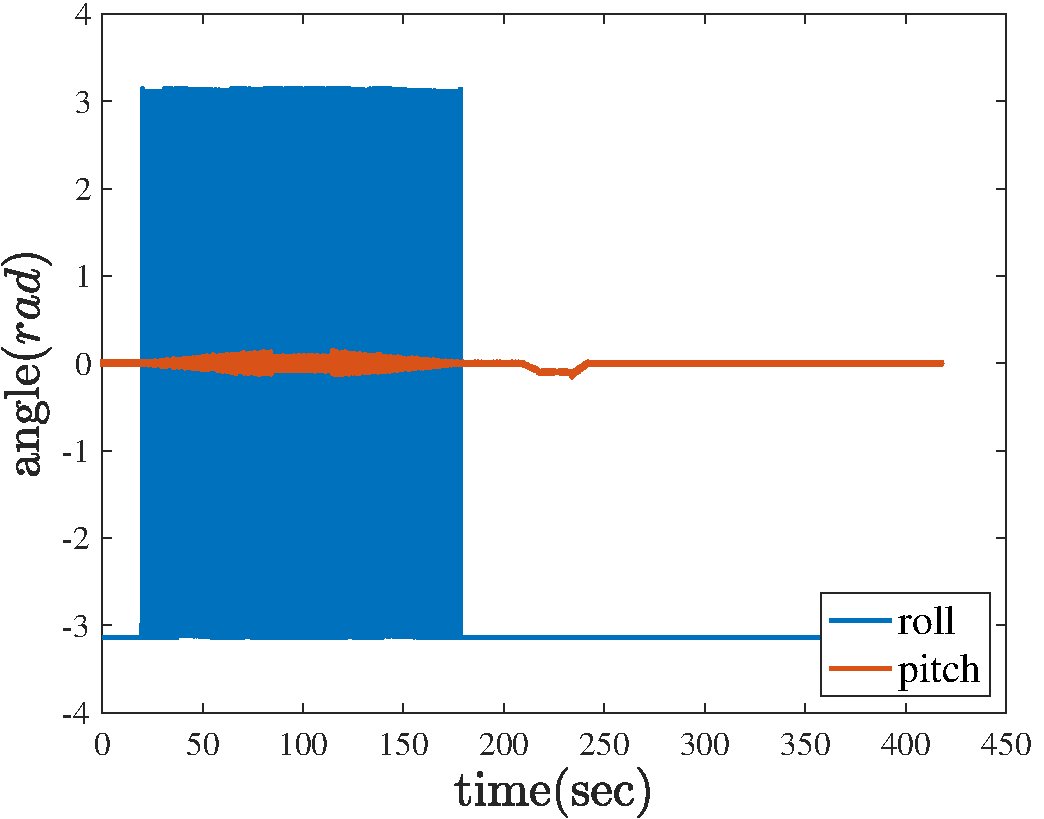
\includegraphics[width=0.8\textwidth]{../Figure/Q1/roll_pitch_2}
  \caption{Roll and pitch angles in scenario II}
  \label{fig:roll_pitch_angles_2}
\end{figure}
\subsection{Collecting data from the gyroscope sensor}
\subsubsection{Gyroscope data rate}
The gyroscope data rate is $0.01$ seconds.

\subsubsection{Gyroscope measurement mechanism in a MEMS accelerometer}
A Microelectromechanical Systems (MEMS) gyroscope is a sensor designed to measure angular velocity. Unlike accelerometers that measure linear acceleration, a gyroscope senses rotational or angular motion.

The gyroscope typically utilizes a vibrating structure, such as a resonating mass or a vibrating ring, which experiences the Coriolis effect when subjected to angular motion. The key steps in the working mechanism are:

\begin{enumerate}
    \item \textbf{Vibrating Structure:} A resonating mass or vibrating ring is employed to initiate a vibration.
    
    \item \textbf{Coriolis Effect:} The Coriolis effect arises when the vibrating structure experiences angular motion. This effect causes the structure to deviate perpendicular to its plane of vibration.
    
    \item \textbf{Sensing the Coriolis Force:} The gyroscope detects the Coriolis force induced by the angular motion. Various sensing mechanisms, such as capacitive or piezoelectric, are commonly used.
    
    \item \textbf{Output Signal:} The detected Coriolis force is translated into an electrical signal, providing an output proportional to the angular velocity of the rotation.
\end{enumerate}

MEMS gyroscopes find applications in navigation systems, robotics, and electronic stability control in vehicles, where precise measurement of angular motion is essential.

\subsubsection{Gyroscope Measures a Body's Angular Velocity Relative to Inertia}

A gyroscope measures a body's angular velocity relative to inertia, denoted as \( \mathbf{w}_{IB} \). This choice is rooted in fundamental principles of rotational dynamics and has several key reasons.

\begin{enumerate}
  \item \textbf{Conservation of Angular Momentum:}
    According to the conservation of angular momentum, the gyroscope measures angular velocity relative to inertia to exploit this principle, providing a reference frame-independent measurement of rotational motion.

  \item \textbf{Inertial Navigation:}
    In applications like inertial navigation systems (INS), precise knowledge of the body's orientation is crucial. Measuring angular velocity relative to inertia allows for accurate navigation calculations.

  \item \textbf{Coordinate System Independence:}
    Measuring angular velocity relative to inertia ensures that the gyroscope output is independent of the orientation of the body, crucial in aerospace and navigation applications.

  \item \textbf{Reference Frame Stability:}
    The inertial frame provides a stable and well-defined reference frame. Measuring relative to inertia ensures consistent and stable angular velocity measurements.

  \item \textbf{Angular Velocity Vector Representation:}
    The angular velocity vector \( \mathbf{v}_{IB} \) represents the rate of change of orientation of the body with respect to the inertial frame, facilitating computations involving rotations and transformations.

  \item \textbf{Compatibility with Integration:}
    Measuring angular velocity relative to inertia simplifies the integration process when obtaining the body's orientation from gyroscope measurements in inertial navigation algorithms.

  \item \textbf{Standardization in Navigation Systems:}
    Standardizing the measurement of angular velocity relative to inertia promotes consistency and interoperability among different systems and devices, especially in navigation and aerospace applications.
\end{enumerate}

\subsubsection{Gyroscope data}
The gyroscope data is shown in the figure \ref{fig:gyroscope_data}.
\begin{figure}[H]
  \centering
  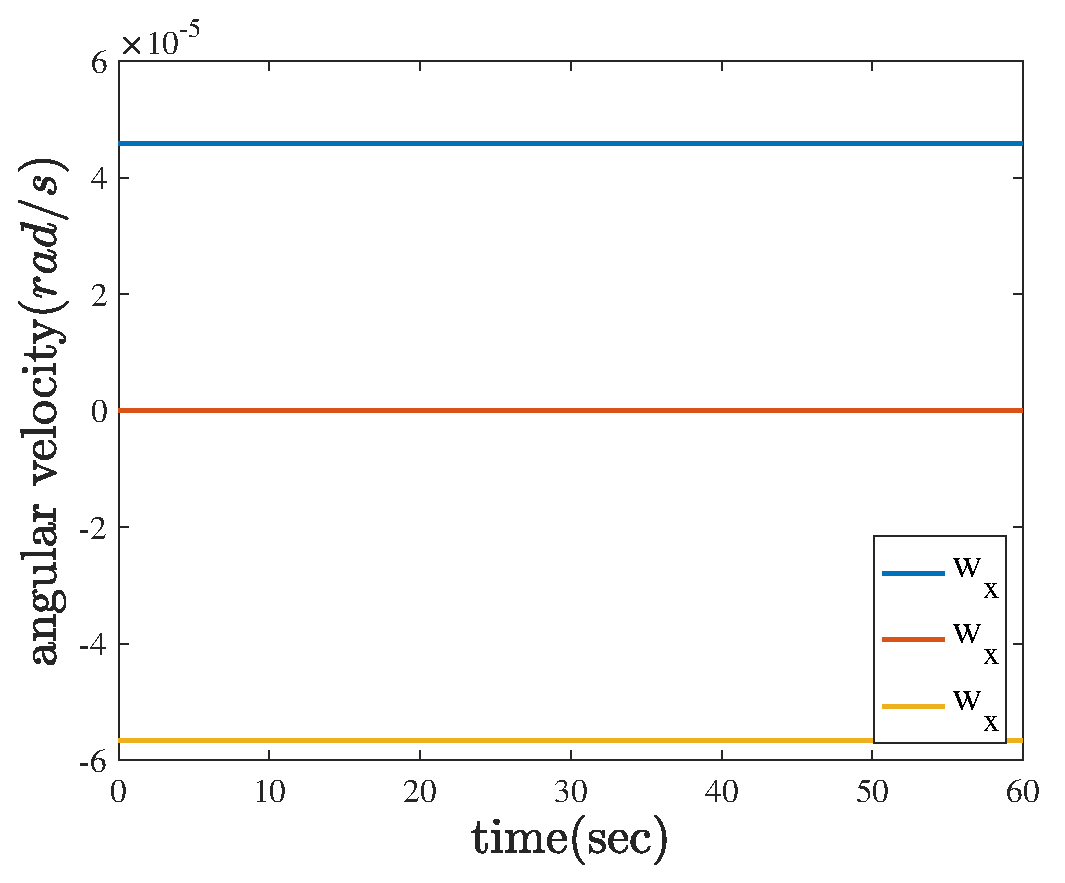
\includegraphics[width=0.8\textwidth]{../Figure/Q1/immovability_w}
  \caption{Gyroscope data}
  \label{fig:gyroscope_data}
\end{figure}

The relationship between Earth's rotation and gyroscope measurement is rooted in the conservation of angular momentum. A gyroscope, when spinning, possesses angular momentum (\(L\)) that tends to maintain its axis of rotation fixed in space. As the Earth rotates, this property influences the behavior of the gyroscope, establishing a significant connection between the two.

The conservation of angular momentum is described by the formula:

\[
L = I \omega
\]

where \(L\) is the angular momentum, \(I\) is the moment of inertia, and \(\omega\) is the angular velocity.


As the Earth rotates, the gyroscope's angular momentum interacts with the Earth's rotation. The gyroscope tends to resist changes in the orientation of its axis, resulting in observable effects. This relationship is harnessed in various applications, including:

\begin{enumerate}
  \item \textbf{Inertial Navigation Systems (INS):} Gyroscopes are integral components of INS, where their measurements provide information about changes in orientation. The Earth's rotation influences these measurements.
\end{enumerate}


\subsection{Collecting data from the magnetometer sensor}
\subsubsection{Magnetometer data rate}
The magnetometer data rate is $0.01$ seconds.
\subsubsection{Yaw angles calibration}
\begin{equation}
  \bm{p} = \bm{m}^B \times \bm{a}^B
\end{equation}
\begin{equation}
  \psi_m = \arctan{\left(\dfrac{p_x}{a_y p_z - a_z p_y}\right)}
\end{equation}

Psi angle is shown in the figure \ref{fig:psi_angle} and \ref{fig:psi_angle_2}.
\begin{figure}[H]
  \centering
  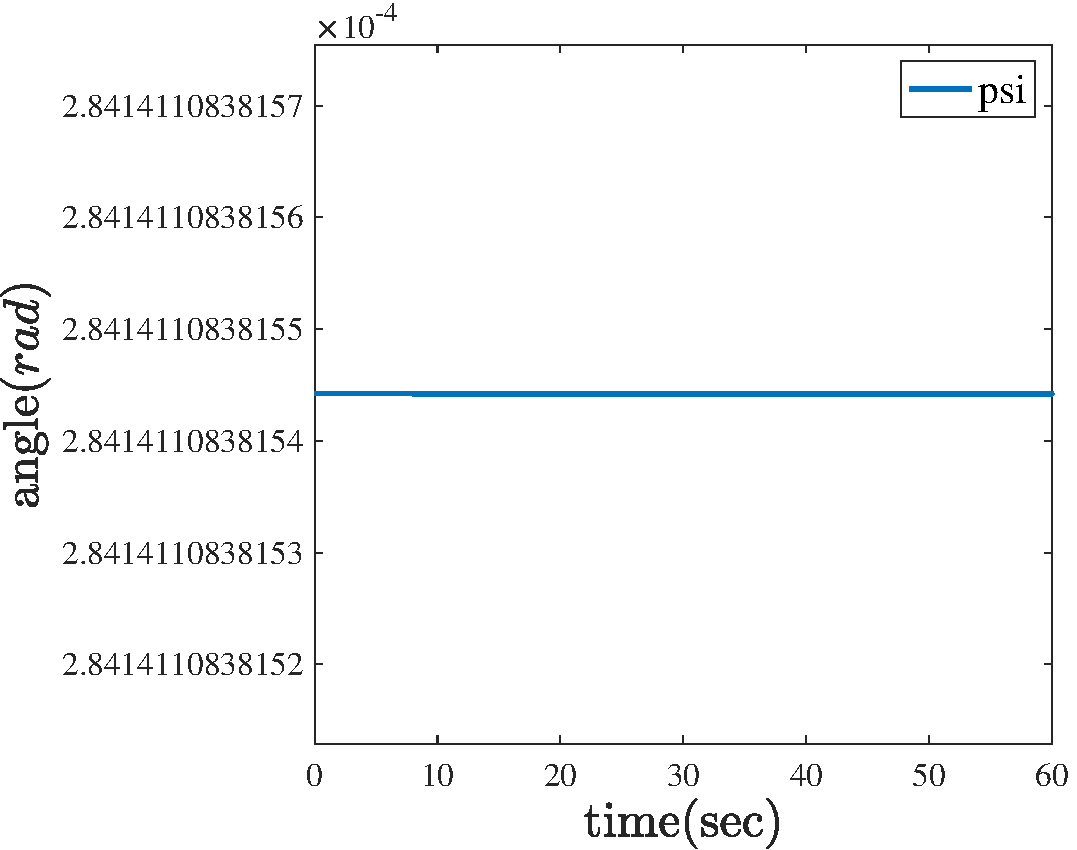
\includegraphics[width=0.8\textwidth]{../Figure/Q1/psi}
  \caption{Psi angle in scenario I}
  \label{fig:psi_angle}
\end{figure}

\begin{figure}[H]
  \centering
  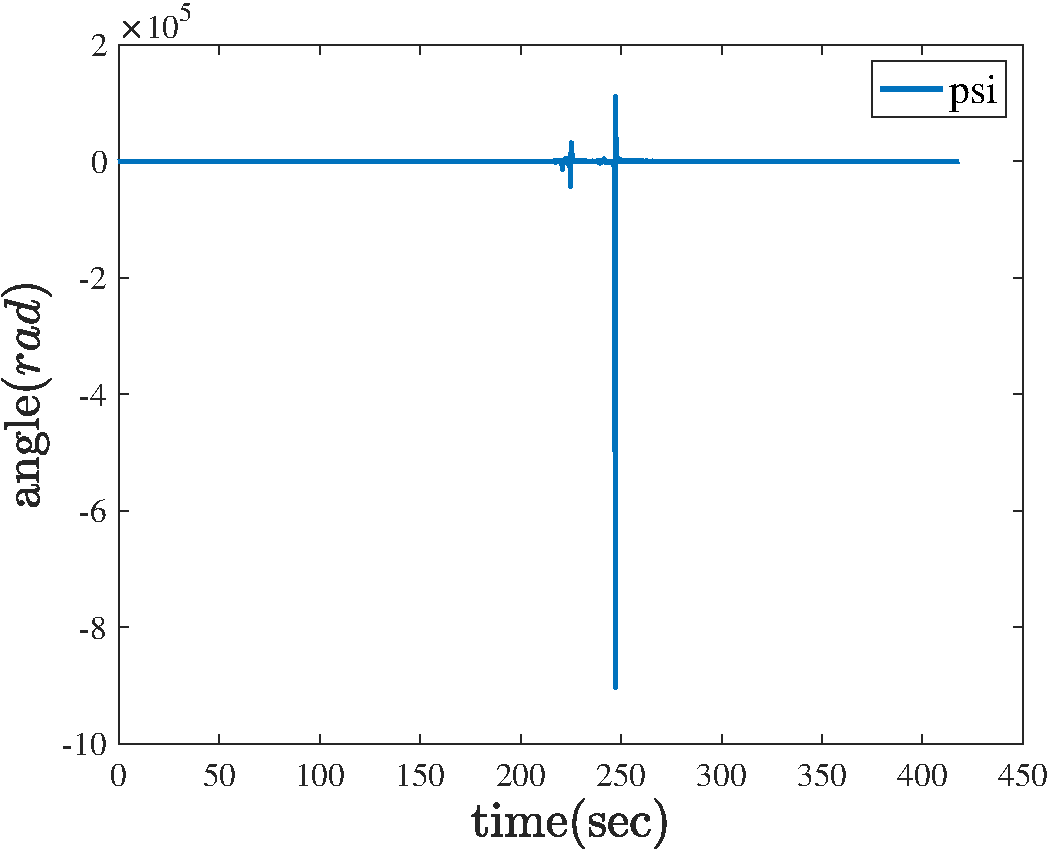
\includegraphics[width=0.8\textwidth]{../Figure/Q1/psi_2}
  \caption{Psi angle in scenario II}
  \label{fig:psi_angle_2}
\end{figure}

\subsection{Collecting data from the GPS sensor}
\subsubsection{GPS data rate}
The gyroscope data rate is $1$ seconds.

\subsubsection{Yas calculation using GPS data}
The yaw angle is calculated using the following equation:
\begin{equation}
  \psi = \arctan{\left(\dfrac{v_e}{v_n}\right)}
\end{equation}

The yaw angle is shown in the figure \ref{fig:psi_angle_gps} and \ref{fig:psi_angle_gps_2}.
\begin{figure}[H]
  \centering
  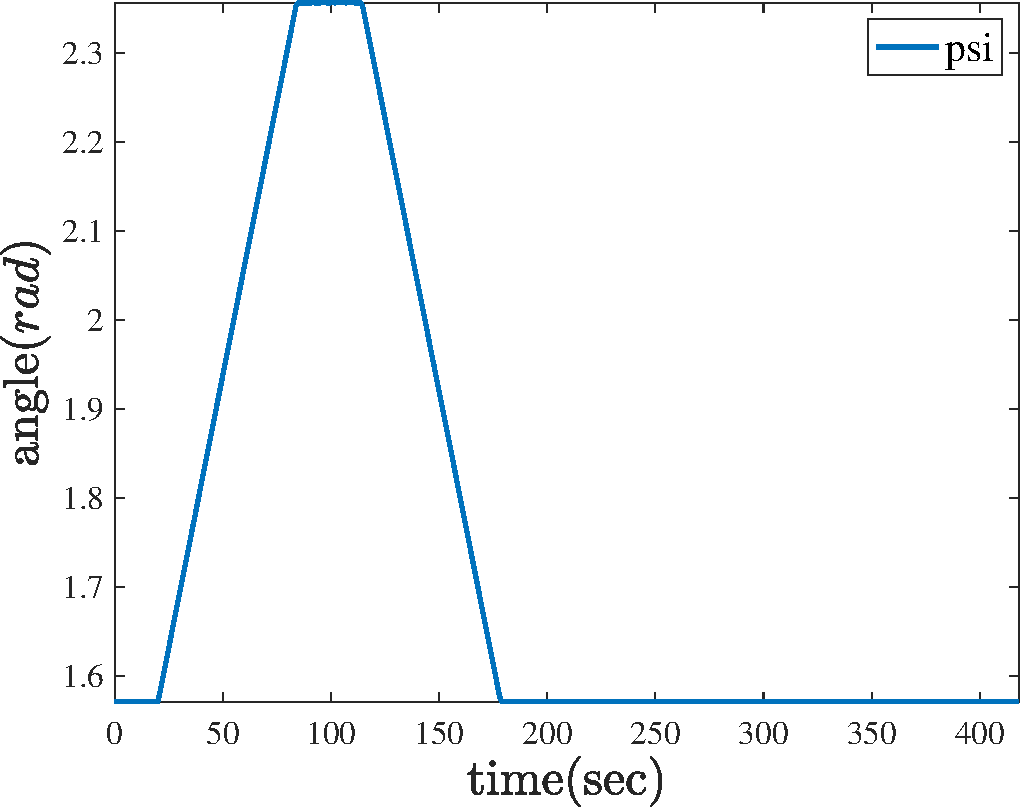
\includegraphics[width=0.8\textwidth]{../Figure/Q1/psi_3}
  \caption{Psi angle in scenario I}
  \label{fig:psi_angle_gps}
\end{figure}

